\documentclass[border=10pt]{standalone}
\usepackage{tikz}
\usetikzlibrary{arrows.meta,positioning,calc,decorations.pathreplacing}
\begin{document}
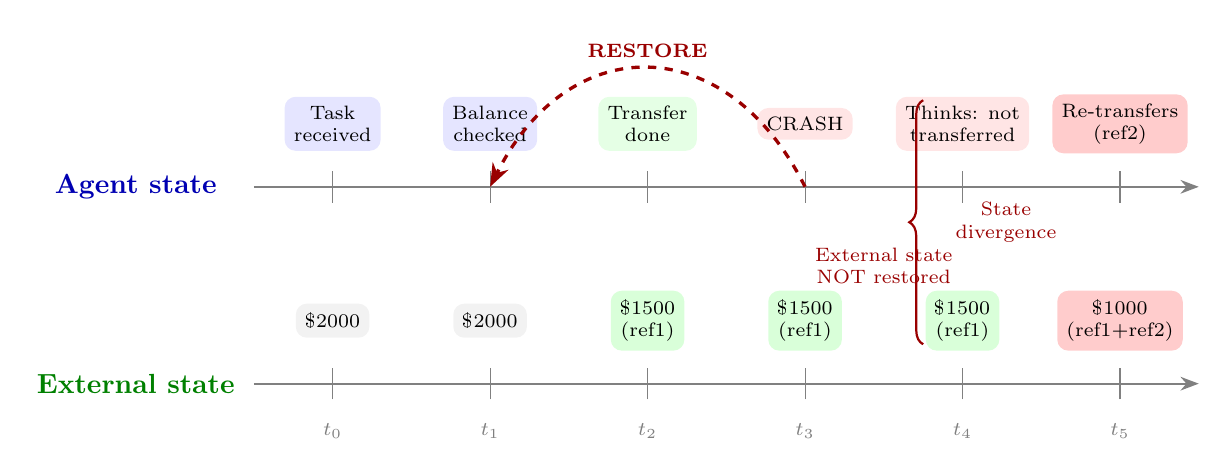
\begin{tikzpicture}[font=\small, >=Stealth]

% Two tracks
\node[font=\bfseries, blue!70!black] at (-1.5, 0.5) {Agent state};
\node[font=\bfseries, green!50!black] at (-1.5, -2) {External state};

% Timeline
\draw[->, thick, gray] (0,0.5) -- (12,0.5);
\draw[->, thick, gray] (0,-2) -- (12,-2);

% Time markers
\foreach \x/\t in {1/t_0, 3/t_1, 5/t_2, 7/t_3, 9/t_4, 11/t_5} {
  \draw[gray] (\x,0.3) -- (\x,0.7);
  \draw[gray] (\x,-2.2) -- (\x,-1.8);
  \node[font=\scriptsize, gray] at (\x, -2.6) {$\t$};
}

% Agent state track
\node[fill=blue!10, rounded corners, font=\scriptsize, align=center] at (1,1.3) {Task\\received};
\node[fill=blue!10, rounded corners, font=\scriptsize, align=center] at (3,1.3) {Balance\\checked};
\node[fill=green!10, rounded corners, font=\scriptsize, align=center] at (5,1.3) {Transfer\\done};
\node[fill=red!10, rounded corners, font=\scriptsize, align=center] at (7,1.3) {CRASH};

% Restore arrow on agent track
\draw[->, very thick, red!60!black, dashed] (7,0.5) .. controls (6,2.5) and (4,2.5) .. node[above, font=\scriptsize\bfseries, red!60!black] {RESTORE} (3,0.5);

% Agent state after restore
\node[fill=red!10, rounded corners, font=\scriptsize, align=center] at (9,1.3) {Thinks: not\\transferred};
\node[fill=red!20, rounded corners, font=\scriptsize, align=center] at (11,1.3) {Re-transfers\\(ref2)};

% External state track
\node[fill=gray!10, rounded corners, font=\scriptsize, align=center] at (1,-1.2) {\$2000};
\node[fill=gray!10, rounded corners, font=\scriptsize, align=center] at (3,-1.2) {\$2000};
\node[fill=green!15, rounded corners, font=\scriptsize, align=center] at (5,-1.2) {\$1500\\(ref1)};
\node[fill=green!15, rounded corners, font=\scriptsize, align=center] at (7,-1.2) {\$1500\\(ref1)};
\node[fill=green!15, rounded corners, font=\scriptsize, align=center] at (9,-1.2) {\$1500\\(ref1)};
\node[fill=red!20, rounded corners, font=\scriptsize, align=center] at (11,-1.2) {\$1000\\(ref1+ref2)};

% No restore on external
\node[font=\scriptsize, red!60!black, align=center] at (8, -0.5) {External state\\NOT restored};

% Divergence brace
\draw[decorate, decoration={brace, amplitude=5pt, mirror}, thick, red!60!black] (8.5,1.6) -- (8.5,-1.5) node[midway, right=8pt, font=\scriptsize, red!60!black, align=center] {State\\divergence};

\end{tikzpicture}
\end{document}
